\documentclass[12pt,letterpaper]{article}
\usepackage[utf8x]{inputenc}
\usepackage{fullpage}
\usepackage[top=2cm, bottom=4.5cm, left=2.5cm, right=2.5cm]{geometry}
\usepackage{amsmath,amsthm,amsfonts,amssymb,amscd}
\usepackage{lastpage}
\usepackage{enumerate}
\usepackage{fancyhdr}
\usepackage{mathrsfs}
\usepackage[svgnames]{xcolor}
\usepackage{graphicx}
\usepackage{listings}
\usepackage{hyperref}
\usepackage{verbatim}
\usepackage{booktabs}
\usepackage{enumitem}
\usepackage{soul}
\usepackage{listings}
\usepackage{titling}
\usepackage{float}
\usepackage{mathtools}
\usepackage{algpseudocode}
\renewcommand\maketitlehooka{\null\mbox{}\vfill}
\renewcommand\maketitlehookd{\vfill\null}
%\renewcommand\thesubsection{\thesection(\alph{subsection})}

\renewcommand{\thesection}{}
\renewcommand{\thesubsection}{\arabic{section}(\alph{subsection})}
\makeatletter
\def\@seccntformat#1{\csname #1ignore\expandafter\endcsname\csname the#1\endcsname\quad}
\let\sectionignore\@gobbletwo
\let\latex@numberline\numberline
\def\numberline#1{\if\relax#1\relax\else\latex@numberline{#1}\fi}
\makeatother

\lstset{language=R,
    basicstyle=\small\ttfamily,
    stringstyle=\color{orange},
    morekeywords={TRUE,FALSE},
    deletekeywords={data,frame,length,as,character},
    keywordstyle=\color{blue},
    commentstyle=\color{magenta},
    showstringspaces=false
}


\hypersetup{%
  colorlinks=true,
  linkcolor=Black,
  linkbordercolor={0 0 1}
}

\setlength{\parindent}{0.0in}
\setlength{\parskip}{0.05in}

% Edit these as appropriate
\newcommand\course{CS 6360.001}
\newcommand\coursename{Database Design}

\newcommand\hwnumber{5}                 % <-- homework number
\newcommand\NetIDa{Ragavalli Ommi (\textit{RXO200000}) \\ Jishnu Jaykumar P (\textit{JJP210003}) \\ Ramya Sarvani Yemineni (\textit{RXY200007})}           % <-- NetID of team members
\newcommand\semester{Fall 2021}           % <-- NetID of person #1
\newcommand{\GroupID}{Team 16}           % <-- Group num for the course

\title{\course, \semester \\ \textbf{\coursename} \\ \vspace{1cm} \Huge Final-Project \\ \GroupID \\ DoorDash-1}
\author{\NetIDa}
\date{}

\begin{document}
\begin{titlingpage}
\maketitle
\end{titlingpage}

\tableofcontents
\newpage
 
\section{Introduction}
This project shows the basic requirements needed for \textbf{DoorDash} food delivery database system. Requirements and functionalities have been figured out via reverse engineering.

\section{Requirements}
\begin{itemize}
    \item DoorDash application is both a web-based as well as a mobile-based application that offers food delivery services to customers.
    \item A person can be registered in the DoorDash application as a customer or a Dasher. (The two roles are disjoint as each role gets a different account. Even if a person is both a customer and dasher, two different accounts would be created based on the roles. Hence, the person entity specialization to customer and dasher would be disjoint.)
    \item A customer can order food from the restaurants of their choice which are in certain proximity with the customer’s location.
    \item A customer can when selected a restaurant will be able to check the menu and different offers offered by that restaurant.
    \item After selecting the food items the customer can pay for the order and will be able to add an additional tip for the delivery service.
    \item The application asks the customer to enter the delivery location and adds a location pin to the order for making the door dasher find the location easily.
    \item The application initially shows the restaurants that are in proximity with the customers location by directly using the GPS location of the customer.
    \item Customers are shown the restaurants that are closed and the opening time for them.
    \item A customer can favorite a restaurant for future quick reference.
    \item Payment methods can be debit / credit card.
    \item The total price of the order includes the cost of the food, taxes and delivery charges which are priced according to the customer’s location and the restaurant’s location.
    \item Each restaurant gets the notification whenever a customer places an order in their restaurant and the restaurant updates the status of the order until it is picked up by the dasher. 
    \item A customer can order food items from a single restaurant at a time, i.e., cannot get food items from multiple restaurants in a single order.
    \item The customer will get a notification after the restaurant has confirmed the order.
    \item The application will let the customer track the live delivery status of the order, i.e., if the order has been picked up or the live location of the dasher.
\end{itemize}
\section{Relationships}
\begin{itemize}
\item Customer-card: One Customer can have multiple cards, and one card can be used by multiple customers (eg. Family members) so the cardinality ratio is M:N.
\item Customer-coupon: One Customer can have multiple coupons, one coupon can be used by multiple users, So the cardinality ratio is M:N.
\item Customer-Address: One Customer can have multiple addresses and One Address can have multiple address, So the cardinality ration is M:N.
\item Customer-Order: One Customer can have multiple orders, So the cardinality ratio is 1:N.
\item Address-Order: One address can have multiple orders, So the cardinality ratio is 1:N.
\item Order-Restaurant: Multiple orders are taken by a single Restaurant, So the cardinality ratio is N:1.
\item Order-FoodItem: One order can have multiple food items, and multiple orders can have multiple food items, so the cardinality ratio is M:N
\item Order-DasherDirectAccount: Multiple Orders can be given to one DasherDirectAccount, so the cardinality ratio is N:1
\item Order-Dasher: Multiple orders can be given to a single Dasher, So the cardinality ratio is N:1.
\item Restaurant-FoodItem: One Restaurant can have multiple food items, and one food item can be in multiple restaurants, so the cardinality ratio is M:N
\item Restaurant-Address: One Restaurant can have a single Address, so the cardinality ratio is 1:1
\item Card-Order: One card can pay for multiple orders, so the cardinality ratio is 1:N
\item Dasher-DasherDirectAccount: One Dasher has only one DasherDirectAccount, so the cardinality ratio is 1:1.
\item Customer-DashPass: One Customer can only have one Dashpass, so the cardinality ratio is 1:1.
\item Order-DashPass: For One order there can be multiple Dashpass used, so the cardinality ratio is 1:N.

\end{itemize}

\section{EER Diagram}
\begin{figure}[H]
 \begin{center}
     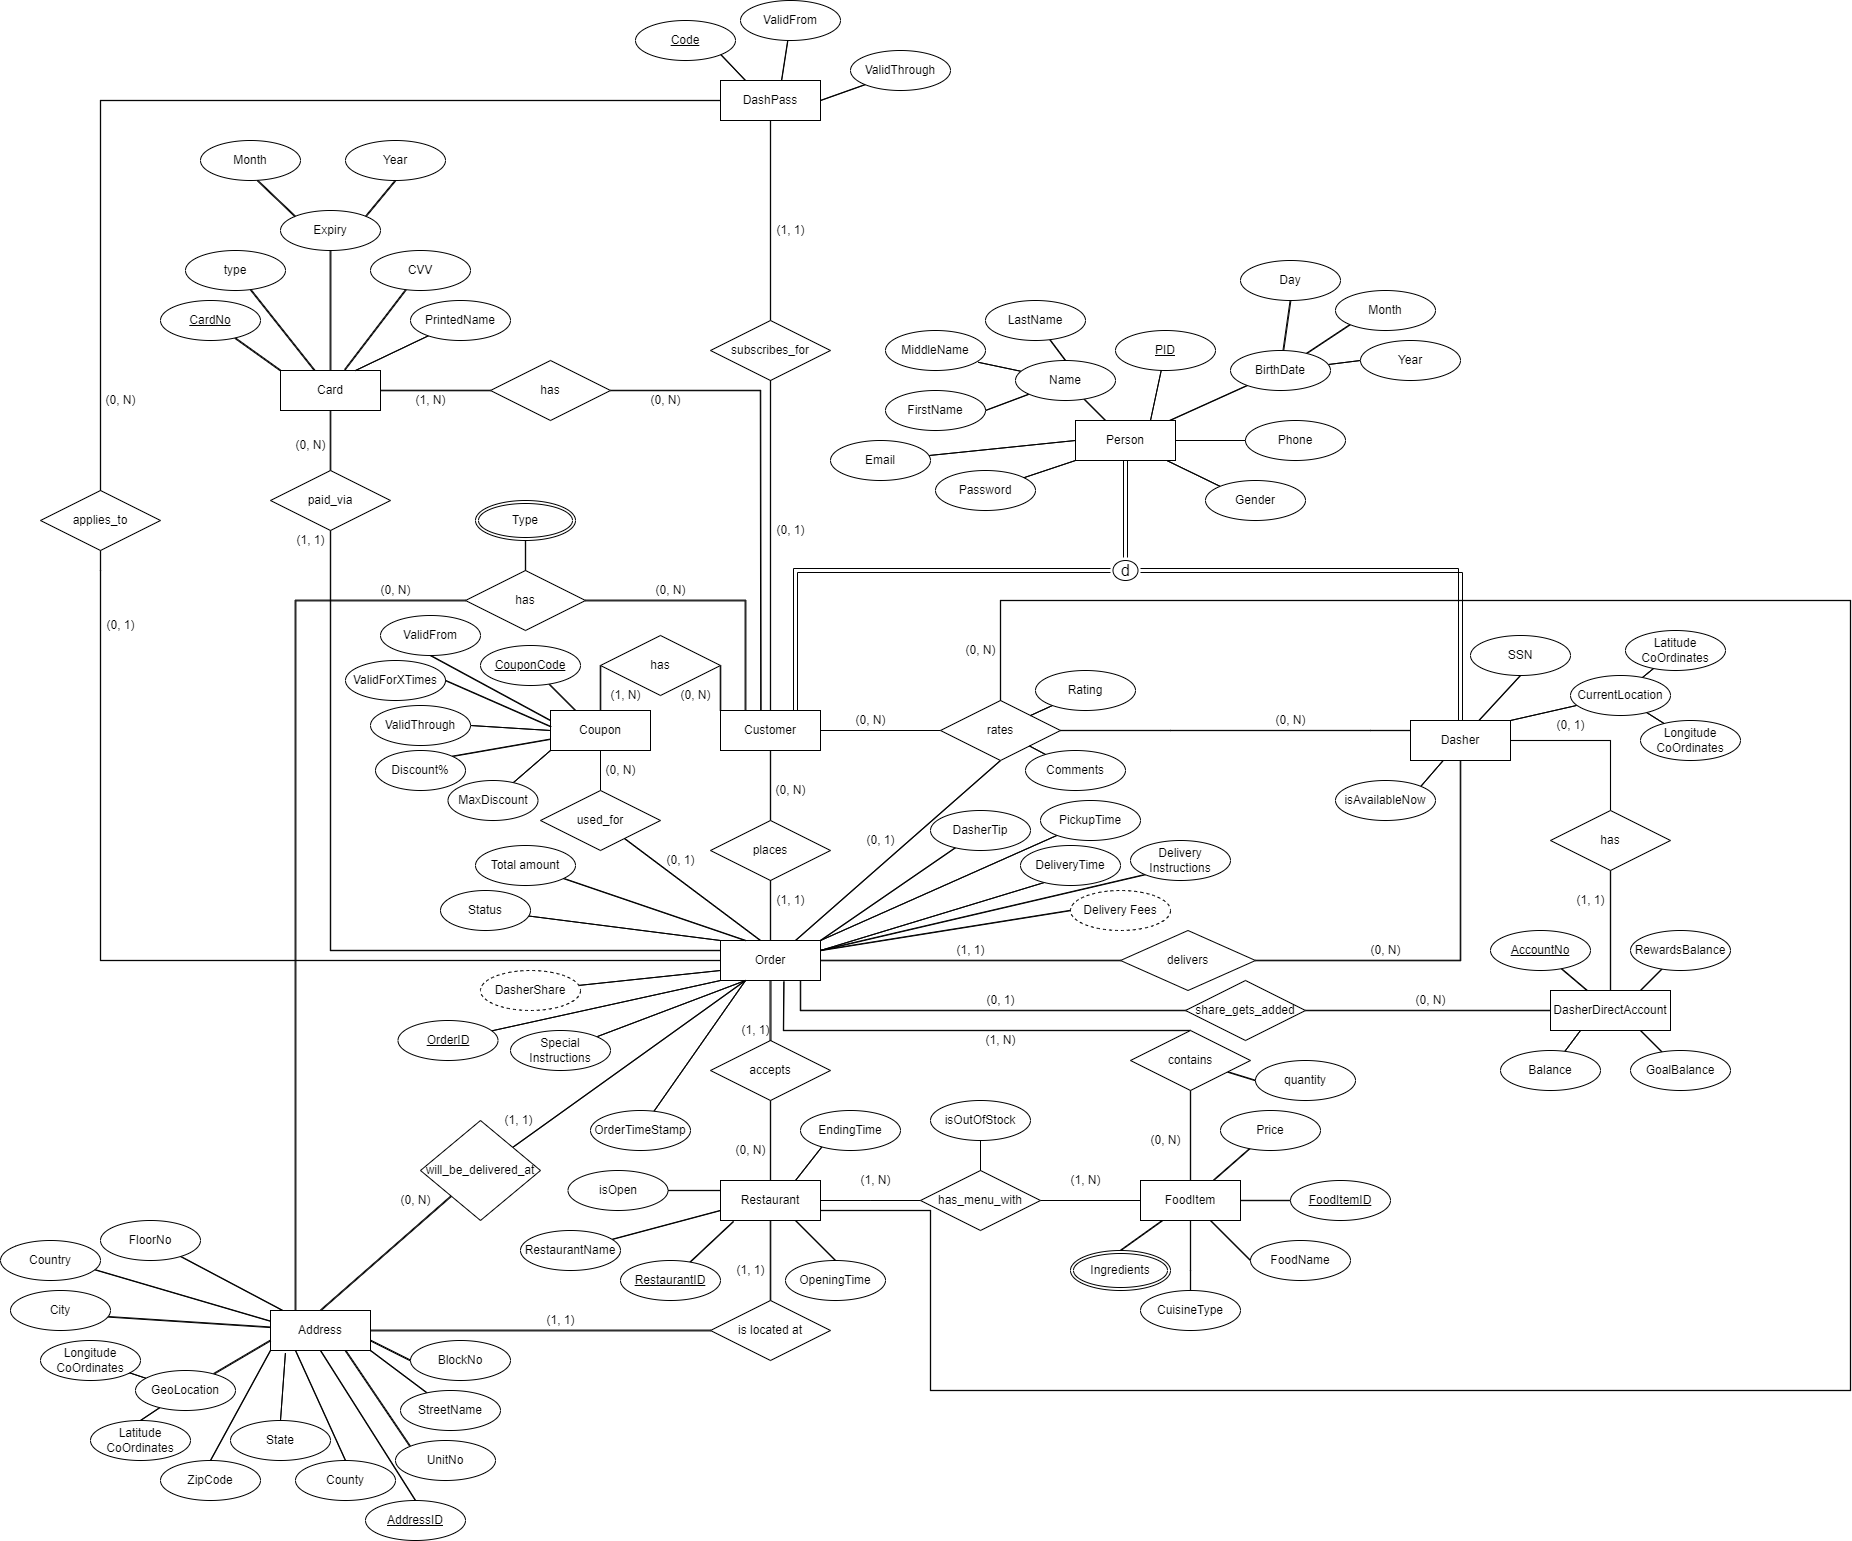
\includegraphics[scale=0.25]{figures/eer.png}
     \caption{EER diagram for our DoorDash food delivery system.}
     \label{fig:eer}
 \end{center}
\end{figure}

\par{Following are the details about the relationships in EER shown in figure:\ref{fig:eer}}
\begin{itemize}
    \item Number of 1:1 relationship = 3
    \item Number of 1:N relationships =  6
    \item Number of M:N relationships =  5
    \item Total number of relationships = 14
\end{itemize}

\section{Relational Model}
\begin{figure}[H]
 \begin{center}
     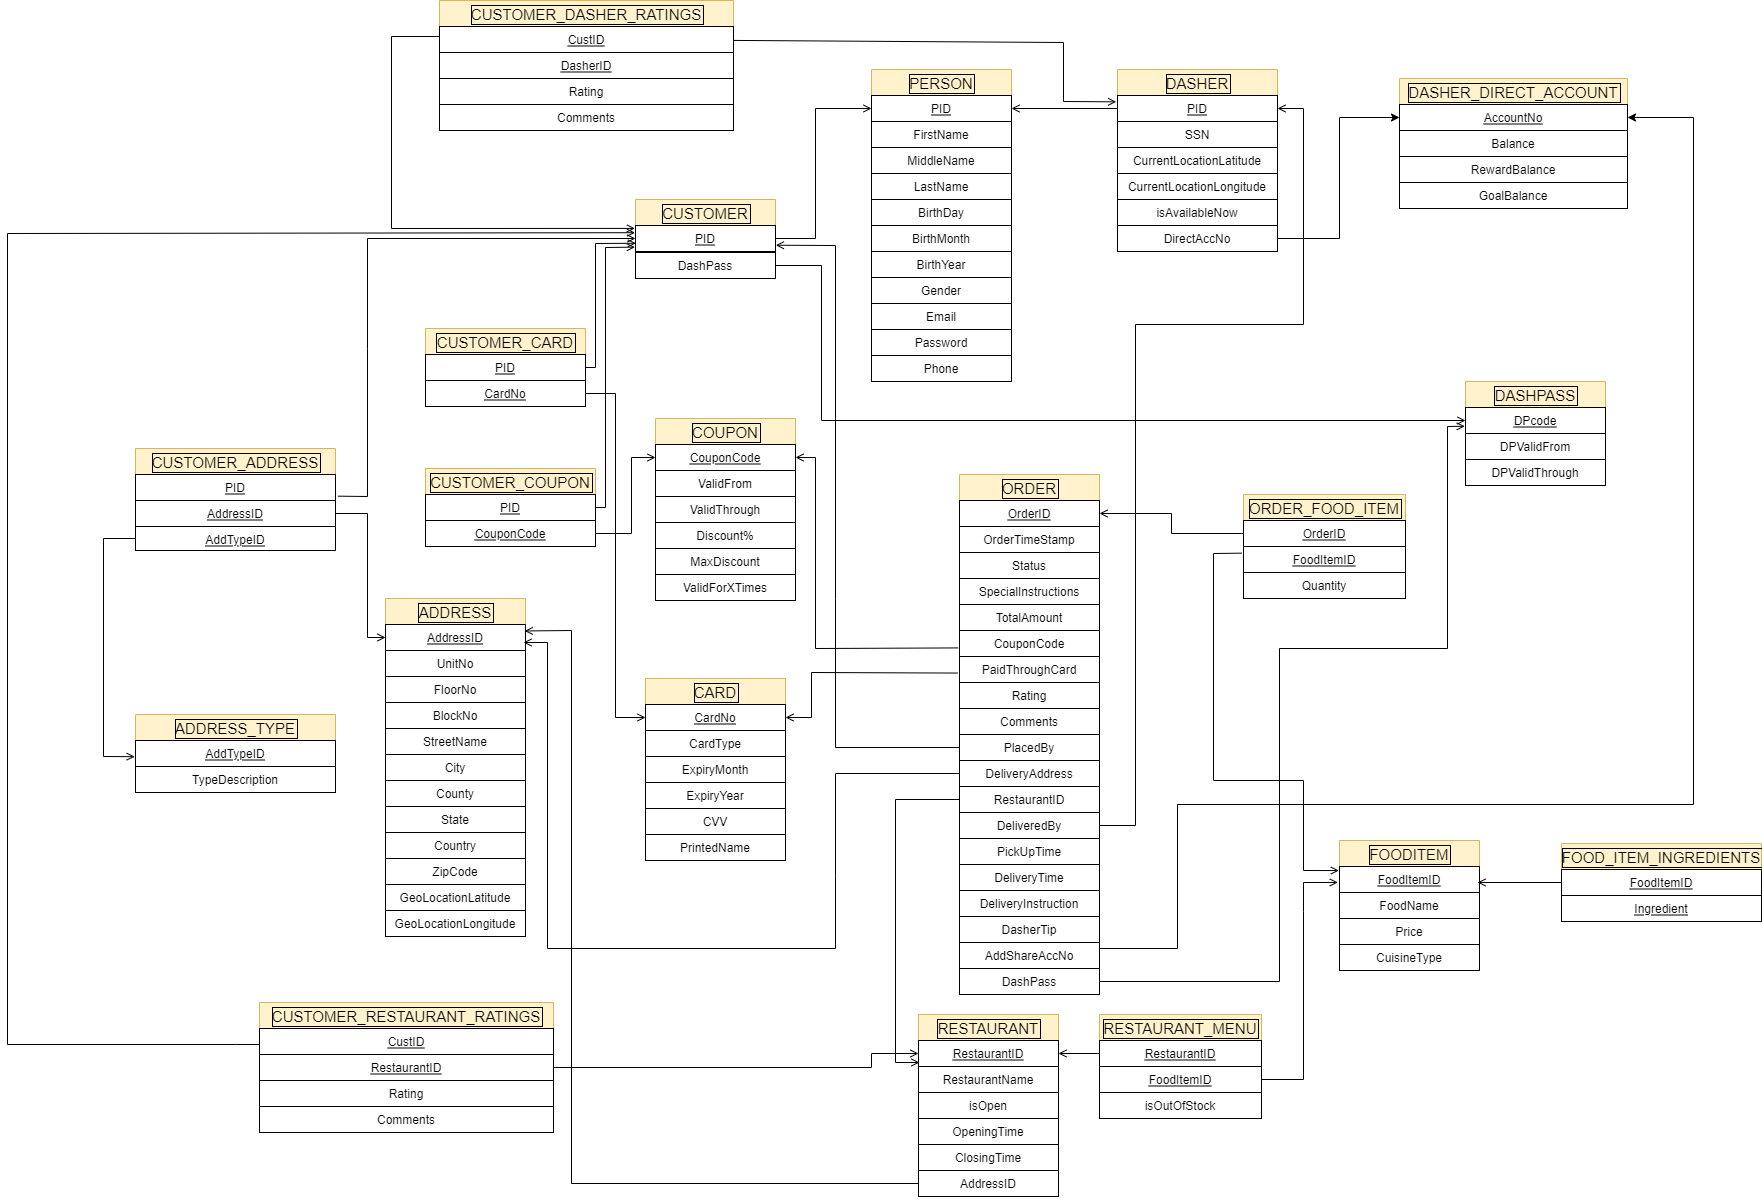
\includegraphics[scale=0.25]{figures/rel-model.png}
     \caption{Relational model made for EER diagram$^{\ref{fig:eer}}$}
     \label{fig:rel-model}
 \end{center}
\end{figure}

\section{Normalization}
The below are the tables that are used in this database which are normalized and does not violate any normalization rules. All the tables above are already in to 3 NF and there are no partial dependencies or transitive dependencies. So, the above relational schema is the final schema.


\begin{figure}[H]
 \begin{center}
     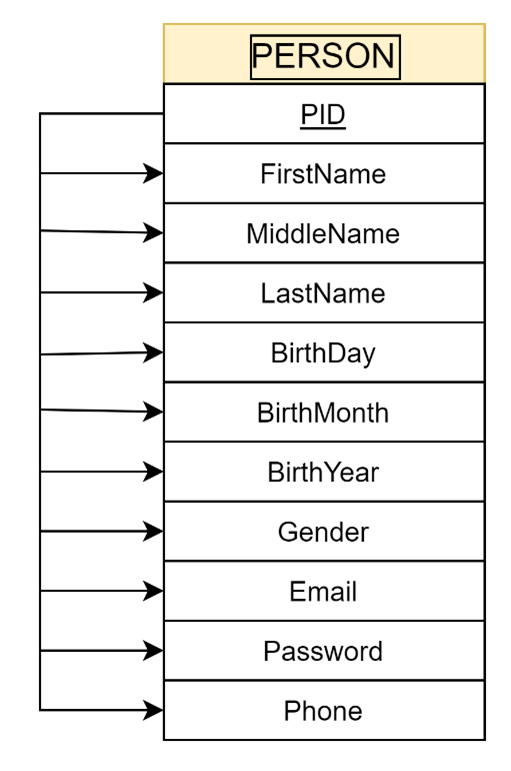
\includegraphics[width=.24\textwidth]{figures/Picture1.png}\hfill
      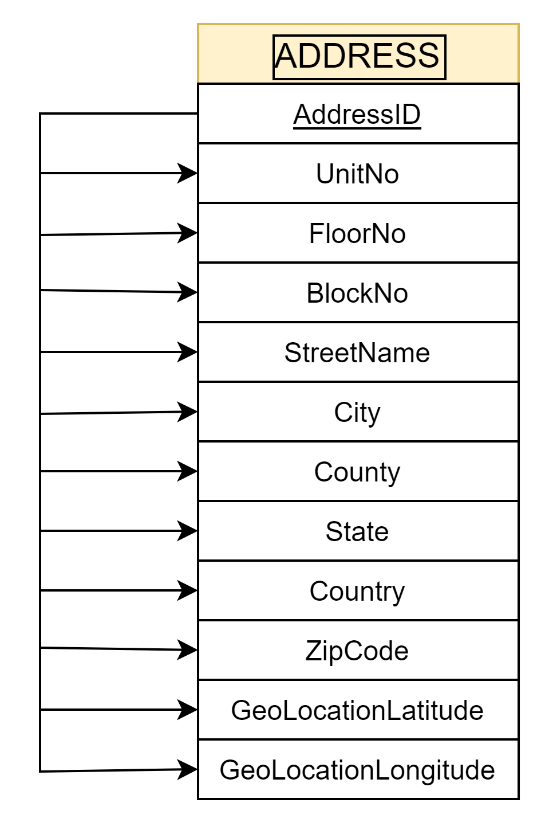
\includegraphics[width=.24\textwidth]{figures/Picture5.png}\hfill
       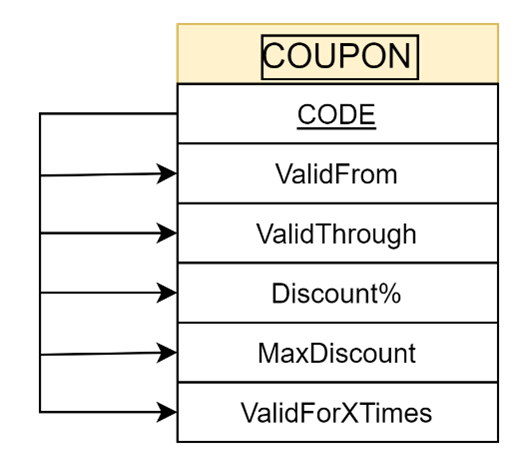
\includegraphics[width=.24\textwidth]{figures/Picture7.png}\hfill
        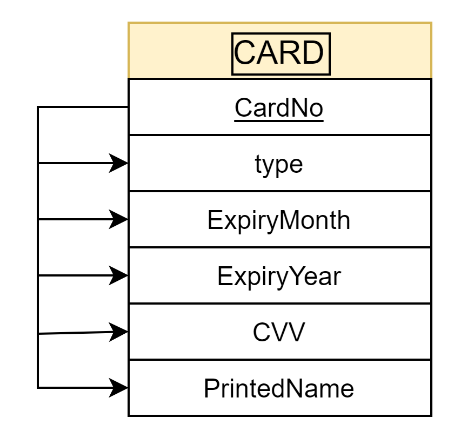
\includegraphics[width=.24\textwidth]{figures/Picture9.png}\hfill
        \\[\smallskipamount]
             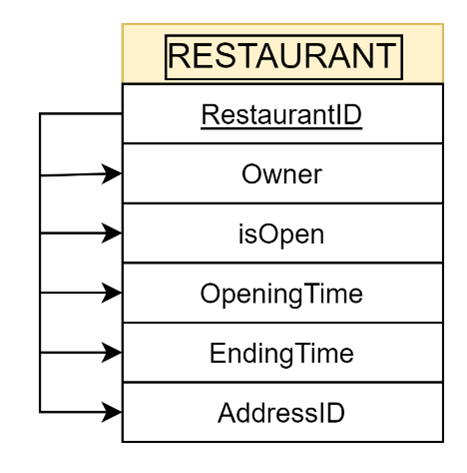
\includegraphics[width=.24\textwidth]{figures/Picture14.png}\hfill
      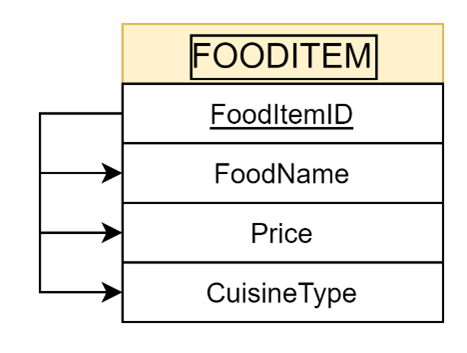
\includegraphics[width=.24\textwidth]{figures/Picture12.png}\hfill
       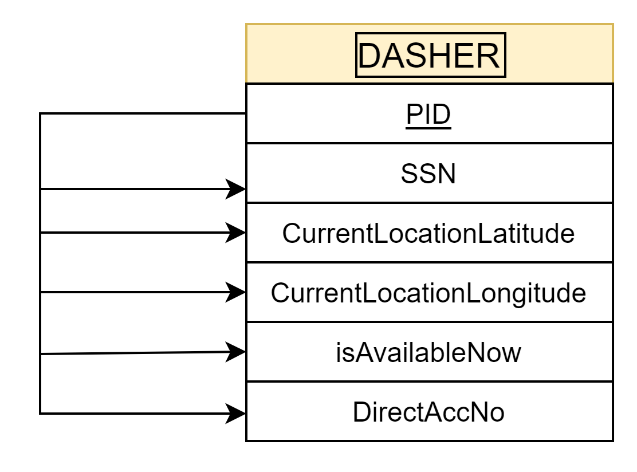
\includegraphics[width=.24\textwidth]{figures/Picture16.png}\hfill
        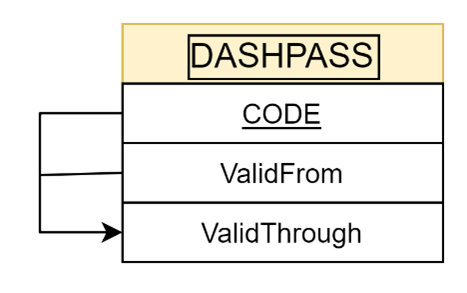
\includegraphics[width=.24\textwidth]{figures/Picture18.png}\hfill
        \\[\smallskipamount]
             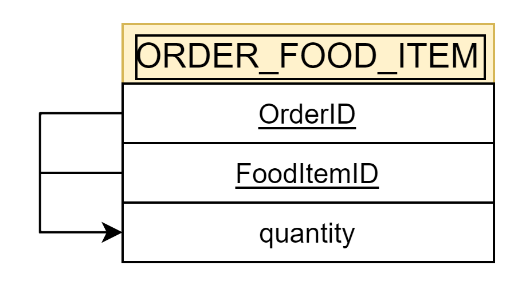
\includegraphics[width=.24\textwidth]{figures/Picture11.png}\hfill
      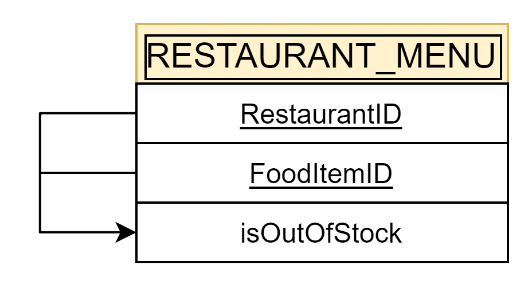
\includegraphics[width=.24\textwidth]{figures/Picture15.png}\hfill
       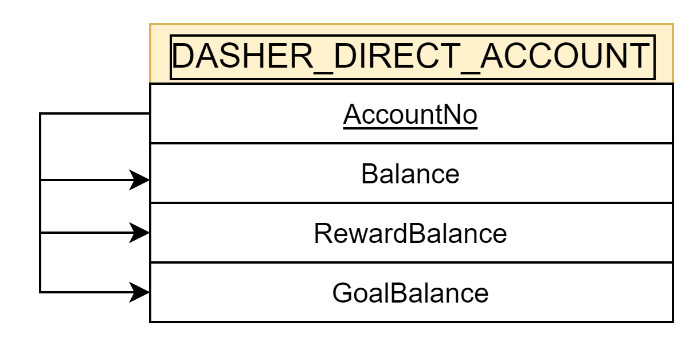
\includegraphics[width=.24\textwidth]{figures/Picture17.png}\hfill
        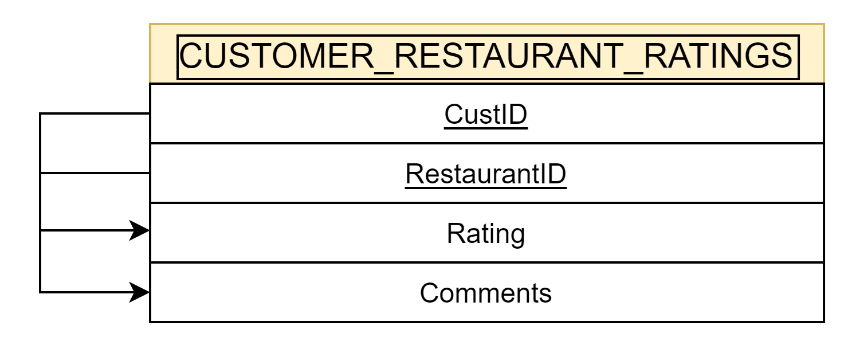
\includegraphics[width=.24\textwidth]{figures/Picture19.png}\hfill
        \\[\smallskipamount]
                 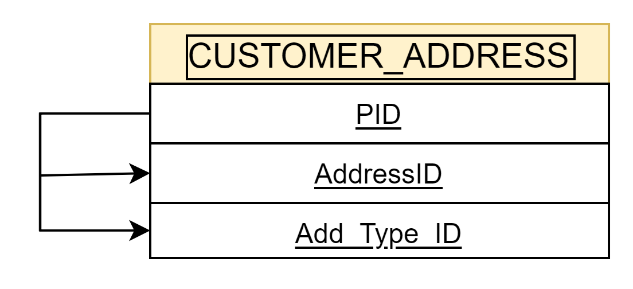
\includegraphics[width=.24\textwidth]{figures/Picture4.png}\hfill
      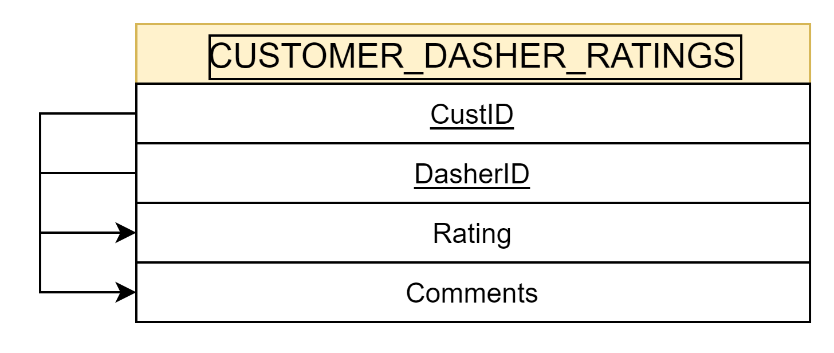
\includegraphics[width=.24\textwidth]{figures/Picture20.png}\hfill
       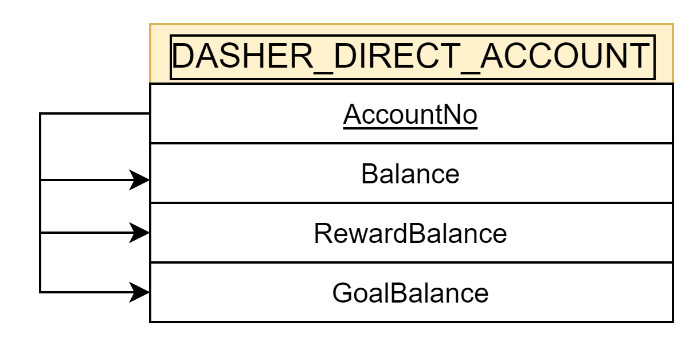
\includegraphics[width=.24\textwidth]{figures/Picture17.png}\hfill
        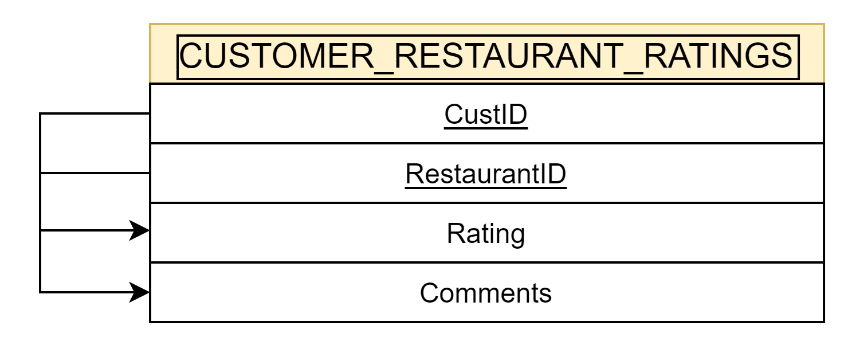
\includegraphics[width=.24\textwidth]{figures/Picture19.png}\hfill
        \\[\smallskipamount]
                     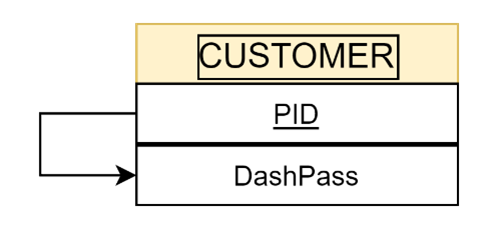
\includegraphics[width=.24\textwidth]{figures/Picture2.png}\hfill
      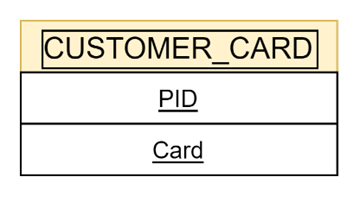
\includegraphics[width=.24\textwidth]{figures/Picture3.png}\hfill
       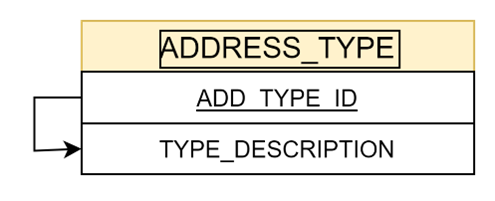
\includegraphics[width=.24\textwidth]{figures/Picture6.png}\hfill
        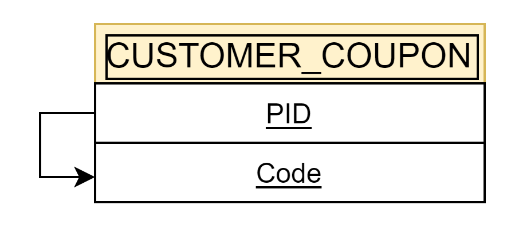
\includegraphics[width=.24\textwidth]{figures/Picture8.png}\hfill
        \\[\smallskipamount]
     \caption{Functional Dependencies (part-1)}
     \label{fig:rel-model-1}
 \end{center}
\end{figure}

\begin{figure}[H]
 \begin{center}
         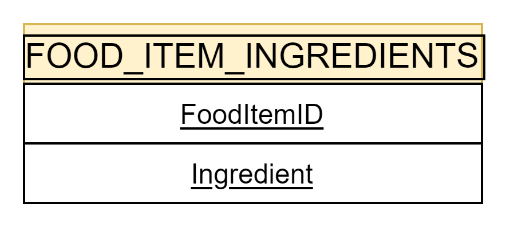
\includegraphics[width=.3\textwidth]{figures/Picture13.png}\hfill
    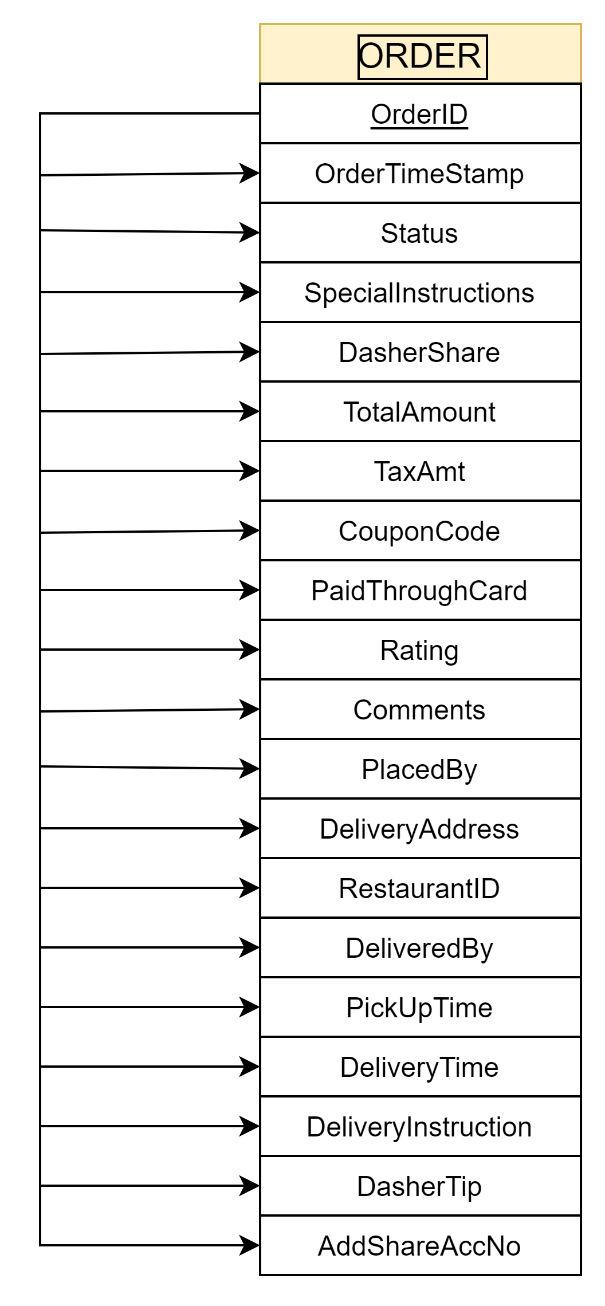
\includegraphics[width=.3\textwidth]{figures/Picture10.png}\hfill
    
     \caption{Functional Dependencies (part-2)}
     \label{fig:rel-model-2}
 \end{center}
\end{figure}


\section{SQL commands}
\subsection*{Create commands}
\begin{lstlisting}
/*Person table*/
CREATE TABLE PERSON (
  PID INTEGER,
  FirstName VARCHAR2(20) NOT NULL,
  MiddleName VARCHAR2(20) DEFAULT NULL,
  LastName VARCHAR2(20) NOT NULL,
  BirthDay INTEGER NOT NULL,
  BirthMonth INTEGER NOT NULL,
  BirthYear INTEGER NOT NULL,
  Gender VARCHAR2(10) NOT NULL,
  Email VARCHAR2(30) NOT NULL,
  Password VARCHAR2(20) NOT NULL,
  Phone CHAR(10) NOT NULL,
  PRIMARY KEY (PID)
);

/*Customer table*/
CREATE TABLE CUSTOMER (
  PID INTEGER,
  DashPass VARCHAR2(10) DEFAULT NULL,
  PRIMARY KEY (PID)
);

/*Dasher table*/
CREATE TABLE DASHER (
  PID INTEGER,
  SSN CHAR(9) NOT NULL,
  CurrentLocationLatitude NUMBER DEFAULT NULL,
  CurrentLocationLongitude NUMBER DEFAULT NULL,
  isAvailableNow VARCHAR2(3) DEFAULT 'Yes',
  DirectAcctNo INTEGER DEFAULT NULL,
  PRIMARY KEY (PID)
);

/*Dashpass table*/
CREATE TABLE DASHPASS (
    DPcode VARCHAR2(10),
    DPValidFrom DATE NOT NULL,
    DPValidThrough DATE NOT NULL,
    PRIMARY KEY (DPcode)
);

/*Dasher Direct Account table*/
CREATE TABLE DASHER_DIRECT_ACCOUNT(
  AccountNo INTEGER,
  Balance NUMBER DEFAULT 0,
  RewardBalance NUMBER DEFAULT 0,
  GoalBalance NUMBER DEFAULT 0,
  PRIMARY KEY (AccountNo)
);

/*Orders table*/
CREATE TABLE ORDERS (
    OrderID INTEGER,
    OrderTimeStamp TIMESTAMP DEFAULT NULL,
    Status VARCHAR2(25) NOT NULL,
    SpecialInstructions VARCHAR2(100) DEFAULT NULL,
    TotalAmount NUMBER NOT NULL,
    CouponCode VARCHAR2(10) DEFAULT NULL,
    PaidThroughCard INTEGER NOT NULL,
    Rating INTEGER DEFAULT NULL,
    Comments VARCHAR2(50) DEFAULT NULL,
    PlacedBy INTEGER NOT NULL,
    DeliveryAddress INTEGER NOT NULL,
    RestaurantID INTEGER NOT NULL,
    DeliveredBy INTEGER NOT NULL,
    PickUpTime TIMESTAMP DEFAULT NULL,
    DeliveryTime TIMESTAMP DEFAULT NULL,
    DeliveryInstruction VARCHAR2(100) DEFAULT NULL,
    DasherTip NUMBER NOT NULL,
    AddShareAccNo INTEGER DEFAULT NULL,
    DashPass VARCHAR2(10) DEFAULT NULL,
    PRIMARY KEY (OrderID)
);

/*Restaurant table*/
CREATE TABLE RESTAURANT (
  RestaurantID INTEGER,
  RestaurantName VARCHAR2(60) NOT NULL,
  isOpen VARCHAR2(3) DEFAULT 'Yes',
  OpeningTime VARCHAR2(20) DEFAULT NULL,
  ClosingTime VARCHAR2(20) DEFAULT NULL,
  AddressID INTEGER NOT NULL,
  PRIMARY KEY (RestaurantID)
);



/*Food item table*/
CREATE TABLE FOODITEM (
  FoodItemID INTEGER,
  FoodName VARCHAR2(100) NOT NULL,
  Price NUMBER NOT NULL,
  CuisineType VARCHAR2(20) DEFAULT NULL,
  PRIMARY KEY (FoodItemID)
);

/*Card table*/
CREATE TABLE CARD (
  CardNo INTEGER,
  CardType VARCHAR2(6) NOT NULL,
  ExpiryMonth INTEGER NOT NULL,
  ExpiryYear INTEGER NOT NULL,
  CVV INTEGER NOT NULL,
  PrintedName VARCHAR2(60) NOT NULL,
  PRIMARY KEY (CardNo)
);

/*Coupon table*/
CREATE TABLE COUPON (
  CouponCode VARCHAR2(10),
  ValidFrom DATE NOT NULL,
  ValidThrough DATE NOT NULL,
  DiscountPercent INTEGER NOT NULL,
  MaxDiscount INTEGER NOT NULL,
  ValidForXTimes INTEGER DEFAULT 1,
  PRIMARY KEY (CouponCode)
);


/*Address table*/
CREATE TABLE ADDRESS (
  AddressID INTEGER,
  UnitNo VARCHAR2(20) DEFAULT NULL,
  FloorNo VARCHAR2(2) DEFAULT NULL,
  BlockNo VARCHAR2(20) DEFAULT NULL,
  StreetName VARCHAR2(40) NOT NULL,
  City VARCHAR2(20) NOT NULL,
  County VARCHAR2(20) DEFAULT NULL,
  State VARCHAR2(20) NOT NULL,
  Country VARCHAR2(20) NOT NULL,
  ZipCode VARCHAR2(10) NOT NULL,
  GeoLocationLatitude NUMBER NOT NULL,
  GeoLocationLongitude NUMBER NOT NULL,
  PRIMARY KEY (AddressID)
);

/* Customer Address Table */
CREATE TABLE CUSTOMER_ADDRESS(
  PID INTEGER,
  AddressID INTEGER,
  AddTypeID INTEGER,
  PRIMARY KEY (PID, AddressID, AddTypeID)
);

/* Address Type Table */
CREATE TABLE ADDRESS_TYPE(
  AddTypeID INTEGER,
  TypeDescription VARCHAR2(10) NOT NULL,
  PRIMARY KEY (AddTypeID)
);

/* Customer Card Table */
CREATE TABLE CUSTOMER_CARD (
  PID INTEGER,
  CardNo INTEGER,
  PRIMARY KEY (PID, CardNo)
);

/* Customer Coupon Table */
CREATE TABLE CUSTOMER_COUPON (
  PID INTEGER,
  CouponCode VARCHAR2(10),
  PRIMARY KEY (PID, CouponCode)
);

/* Order Food Item Table */
CREATE TABLE ORDER_FOOD_ITEM (
  OrderID INTEGER,
  FoodItemID INTEGER,
  Quantity INTEGER NOT NULL,
  PRIMARY KEY (OrderID, FoodItemID)
);

/* Restaurant Menu Table */
CREATE TABLE RESTAURANT_MENU (
  RestaurantID INTEGER,
  FoodItemID INTEGER,
  isOutofStock VARCHAR2(3) DEFAULT 'No',
  PRIMARY KEY (RestaurantID, FoodItemID)
);

/* Food Item Ingredients Table */
CREATE TABLE FOOD_ITEM_INGREDIENTS (
  FoodItemID INTEGER,
  Ingredient VARCHAR2(50),
  PRIMARY KEY (FoodItemID, Ingredient)
);

/* Customer Dasher Ratings */
CREATE TABLE CUSTOMER_DASHER_RATINGS (
    CustID INTEGER,
    DasherID INTEGER,
    Rating INTEGER DEFAULT NULL,
    Comments VARCHAR2(50) DEFAULT NULL,
    PRIMARY KEY (CustID, DasherID)
);

/* Customer Dasher Ratings */
CREATE TABLE CUSTOMER_RESTAURANT_RATINGS (
    CustID INTEGER,
    RestaurantID INTEGER,
    Rating INTEGER DEFAULT NULL,
    Comments VARCHAR2(50) DEFAULT NULL,
    PRIMARY KEY (CustID, RestaurantID)
);

/* Foreign Key constraints */
ALTER TABLE CUSTOMER ADD CONSTRAINT fkcuspid 
FOREIGN KEY(PID) REFERENCES PERSON(PID) ON DELETE CASCADE;

ALTER TABLE CUSTOMER ADD CONSTRAINT fkcusdashpass 
FOREIGN KEY(DashPass) REFERENCES DASHPASS(DPcode) ON DELETE SET NULL;

ALTER TABLE DASHER ADD CONSTRAINT fkdaspid 
FOREIGN KEY(PID) REFERENCES PERSON(PID) ON DELETE CASCADE;

ALTER TABLE DASHER ADD CONSTRAINT fkdasacct 
FOREIGN KEY(DirectAcctNo) REFERENCES DASHER_DIRECT_ACCOUNT(AccountNo) 
ON DELETE SET NULL;

ALTER TABLE CUSTOMER_ADDRESS ADD CONSTRAINT fkcusaddpid 
FOREIGN KEY(PID) REFERENCES CUSTOMER(PID) ON DELETE CASCADE;

ALTER TABLE CUSTOMER_ADDRESS ADD CONSTRAINT fkaddid 
FOREIGN KEY(AddressID) REFERENCES ADDRESS(AddressID) 
ON DELETE CASCADE;

ALTER TABLE CUSTOMER_ADDRESS ADD CONSTRAINT fkaddtypeid 
FOREIGN KEY(AddTypeID) REFERENCES ADDRESS_TYPE(AddTypeID) 
ON DELETE CASCADE;

ALTER TABLE CUSTOMER_CARD ADD CONSTRAINT fkcuscardpid 
FOREIGN KEY(PID) REFERENCES CUSTOMER(PID) ON DELETE CASCADE;

ALTER TABLE CUSTOMER_CARD ADD CONSTRAINT fkcuscardno 
FOREIGN KEY(CardNo) REFERENCES CARD(CardNo) ON DELETE CASCADE;

ALTER TABLE CUSTOMER_COUPON ADD CONSTRAINT fkcuscouppid 
FOREIGN KEY(PID) REFERENCES CUSTOMER(PID) ON DELETE CASCADE;

ALTER TABLE CUSTOMER_COUPON ADD CONSTRAINT fkcuscoupcode 
FOREIGN KEY(CouponCode) REFERENCES COUPON(CouponCode) 
ON DELETE CASCADE;

ALTER TABLE ORDERS ADD CONSTRAINT fkordcoupcode 
FOREIGN KEY(CouponCode) REFERENCES COUPON(CouponCode) 
ON DELETE SET NULL;

ALTER TABLE ORDERS ADD CONSTRAINT fkordcardno 
FOREIGN KEY(PaidThroughCard) REFERENCES CARD(CardNo) 
ON DELETE SET NULL;

ALTER TABLE ORDERS ADD CONSTRAINT fkordcuspid 
FOREIGN KEY(PlacedBy) REFERENCES CUSTOMER(PID) 
ON DELETE CASCADE;

ALTER TABLE ORDERS ADD CONSTRAINT fkordaddrid 
FOREIGN KEY(DeliveryAddress) REFERENCES ADDRESS(AddressID) 
ON DELETE SET NULL;

ALTER TABLE ORDERS ADD CONSTRAINT fkordresid 
FOREIGN KEY(RestaurantID) REFERENCES RESTAURANT(RestaurantID) 
ON DELETE SET NULL;

ALTER TABLE ORDERS ADD CONSTRAINT fkorddelpid 
FOREIGN KEY(DeliveredBy) REFERENCES DASHER(PID) 
ON DELETE SET NULL;

ALTER TABLE ORDERS ADD CONSTRAINT fkorddashacct 
FOREIGN KEY(AddShareAccNo) REFERENCES DASHER_DIRECT_ACCOUNT(AccountNo) 
ON DELETE SET NULL;

ALTER TABLE ORDERS ADD CONSTRAINT fkorddashpass 
FOREIGN KEY(DashPass) REFERENCES DASHPASS(DPcode) 
ON DELETE SET NULL;

ALTER TABLE RESTAURANT ADD CONSTRAINT fkresaddrid 
FOREIGN KEY(AddressID) REFERENCES ADDRESS(AddressID) 
ON DELETE CASCADE;

ALTER TABLE RESTAURANT_MENU ADD CONSTRAINT fkresmenuid 
FOREIGN KEY(RestaurantID) REFERENCES RESTAURANT(RestaurantID) 
ON DELETE CASCADE;

ALTER TABLE RESTAURANT_MENU ADD CONSTRAINT fkresmenufoodid 
FOREIGN KEY(FoodItemID) REFERENCES FOODITEM(FoodItemID) 
ON DELETE CASCADE;

ALTER TABLE ORDER_FOOD_ITEM ADD CONSTRAINT fkordfoodid 
FOREIGN KEY(OrderID) REFERENCES ORDERS(OrderID) ON DELETE CASCADE;

ALTER TABLE ORDER_FOOD_ITEM ADD CONSTRAINT fkordfooditemid 
FOREIGN KEY(FoodItemID) REFERENCES FOODITEM(FoodItemID) 
ON DELETE CASCADE;

ALTER TABLE FOOD_ITEM_INGREDIENTS ADD CONSTRAINT fkfooditemingid 
FOREIGN KEY(FoodItemID) REFERENCES FOODITEM(FoodItemID) 
ON DELETE CASCADE;

ALTER TABLE CUSTOMER_DASHER_RATINGS ADD CONSTRAINT fkcusrate 
FOREIGN KEY(CustID) REFERENCES CUSTOMER(PID) ON DELETE CASCADE;

ALTER TABLE CUSTOMER_DASHER_RATINGS ADD CONSTRAINT fkdashrate 
FOREIGN KEY(DasherID) REFERENCES DASHER(PID) ON DELETE CASCADE;

ALTER TABLE CUSTOMER_RESTAURANT_RATINGS ADD CONSTRAINT fkcusrate1 
FOREIGN KEY(CustID) REFERENCES CUSTOMER(PID) ON DELETE CASCADE;

ALTER TABLE CUSTOMER_RESTAURANT_RATINGS ADD CONSTRAINT fkresrate 
FOREIGN KEY(RestaurantID) REFERENCES RESTAURANT(RestaurantID) 
ON DELETE CASCADE;

\end{lstlisting}

\subsection*{Insert Commands}
\begin{lstlisting}
/* Inserting values into the tables */
INSERT INTO person
VALUES     (1,
            'Jon',
            'S',
            'Snow',
            1,
            3,
            1994,
            'Male',
            'jonssnow@gmail.com',
            'JSS@131994',
            '3413562686');

INSERT INTO person
VALUES     (2,
            'Shawn',
            NULL,
            'Mendes',
            27,
            3,
            1994,
            'Male',
            'shawnmendes@gmail.com',
            'SM@2731994',
            '4418566696');

INSERT INTO person
VALUES     (3,
            'Alexis',
            NULL,
            'Martinez',
            8,
            9,
            1996,
            'Female',
            'alexismartinez@gmail.com',
            'AM@891996',
            '2613592688');

INSERT INTO person
VALUES     (4,
            'Camilla',
            'Alaxendra',
            'Cabeyo',
            1,
            9,
            1999,
            'Female',
            'camillaac@gmail.com',
            'CAC@191999',
            '9717592755');

INSERT INTO person
VALUES     (5,
            'Shawn',
            NULL,
            'Mendes',
            27,
            3,
            1994,
            'Male',
            'shawnmendes@gmail.com',
            'SM@2731994',
            '4418566696');

INSERT INTO dashpass
VALUES     ('abc123',
            To_date(sysdate),
            To_date(sysdate) + 30);

INSERT INTO customer
VALUES     (1,
            'abc123');

INSERT INTO customer
VALUES     (2,
            NULL);

INSERT INTO customer
VALUES     (3,
            NULL);

INSERT INTO dasher_direct_account
VALUES     (32391321226,
            30.99,
            2.75,
            300);

INSERT INTO dasher_direct_account
VALUES     (43402432337,
            100.99,
            5.75,
            500);

INSERT INTO dasher
VALUES     (4,
            '123456789',
            NULL,
            NULL,
            'No',
            32391321226);

INSERT INTO dasher
VALUES     (5,
            '987654321',
            52.28220,
            79.41890,
            'Yes',
            43402432337);

INSERT INTO customer_dasher_ratings
VALUES     (1,
            4,
            NULL,
            NULL);

INSERT INTO address
VALUES     (4001,
            NULL,
            NULL,
            NULL,
            '3415 Smithfield Avenue',
            'Lubbock',
            'Dallas',
            'Texas',
            'United States',
            '79401',
            6.54141,
            48.28978);

INSERT INTO address
VALUES     (4002,
            15,
            2,
            1522,
            '800 W Renner Rd',
            'Richardson',
            'Houston',
            'Texas',
            'United States',
            '75020',
            27.11515,
            8.05562);

INSERT INTO address
VALUES     (4003,
            NULL,
            NULL,
            NULL,
            '4605 High Meadow Lane',
            'Lubbock',
            NULL,
            'Texas',
            'United States',
            '75166',
            40.80081,
            165.77609);

INSERT INTO address
VALUES     (4004,
            NULL,
            NULL,
            NULL,
            '2806 Weir Crescent',
            'Lubbock',
            NULL,
            'Texas',
            'United States',
            '75021',
            1.19981,
            108.06388);

INSERT INTO address
VALUES     (4005,
            NULL,
            NULL,
            NULL,
            '4205 Derry Rd',
            'Houston',
            NULL,
            'Texas',
            'United States',
            '75022',
            26.75989,
            161.23763);

INSERT INTO address
VALUES     (4006,
            NULL,
            NULL,
            NULL,
            '4517 Orchard Street',
            'Houston',
            'Houston',
            'Texas',
            'United States',
            '75011',
            37.11515,
            18.05562);

INSERT INTO restaurant
VALUES     (3001,
            'Halal Shack',
            'Yes',
            '10:00:00',
            '05:00:00',
            4003);

INSERT INTO restaurant
VALUES     (3002,
            'Starbucks',
            'Yes',
            '08:00:00',
            '22:00:00',
            4004);

INSERT INTO restaurant
VALUES     (3003,
            'FireHouse Subs',
            'Yes',
            '08:00:00',
            '15:00:00',
            4006);

INSERT INTO restaurant
VALUES     (3004,
            'Supreme Pizza',
            'Yes',
            '10:00:00',
            '17:00:00',
            4005);

INSERT INTO customer_restaurant_ratings
VALUES     (1,
            3001,
            NULL,
            NULL);

INSERT INTO card
VALUES     (4024007101499563,
            'Credit',
            5,
            2025,
            465,
            'Jon S Snow');

INSERT INTO card
VALUES     (4716187198567622,
            'Debit',
            5,
            2024,
            413,
            'Shawn Mendes');

INSERT INTO card
VALUES     (5528494234557053,
            'Credit',
            11,
            2027,
            543,
            'Jon S Snow');

INSERT INTO card
VALUES     (5589278764521597,
            'Debit',
            4,
            2022,
            879,
            'Ragavalli Ommi');

INSERT INTO card
VALUES     (4749050146695161,
            'Debit',
            12,
            2028,
            655,
            'Alia Bhatt');

INSERT INTO coupon
VALUES     ('vYh4x09z',
            date '2021-12-08',
            date '2021-12-31',
            20,
            10,
            10);

INSERT INTO coupon
VALUES     ('3pWRH0Hc',
            date '2021-12-08',
            date '2021-12-31',
            50,
            15,
            1);

INSERT INTO coupon
VALUES     ('JNwKD8Ud',
            date '2021-12-08',
            date '2022-12-08',
            5,
            5,
            5);

INSERT INTO orders
VALUES     (2001,
            timestamp '2021-12-07 12:30:00',
            'Prepared',
            NULL,
            24.39,
            'vYh4x09z',
            4024007101499563,
            3,
            NULL,
            1,
            4001,
            3001,
            4,
            NULL,
            NULL,
            NULL,
            2,
            32391321226,
            NULL);

INSERT INTO orders
VALUES     (2002,
            timestamp '2021-12-06 12:30:00',
            'Prepared',
            NULL,
            24.39,
            'vYh4x09z',
            4024007101499563,
            3,
            NULL,
            1,
            4001,
            3001,
            4,
            NULL,
            NULL,
            NULL,
            2,
            32391321226,
            NULL);

INSERT INTO orders
VALUES     (2003,
            timestamp '2021-12-05 12:30:00',
            'Prepared',
            NULL,
            24.39,
            'vYh4x09z',
            4024007101499563,
            3,
            NULL,
            1,
            4001,
            3001,
            4,
            NULL,
            NULL,
            NULL,
            2,
            32391321226,
            NULL);

INSERT INTO orders
VALUES     (2004,
            timestamp '2021-11-11 12:30:00',
            'Prepared',
            NULL,
            24.39,
            'vYh4x09z',
            4024007101499563,
            3,
            NULL,
            1,
            4001,
            3001,
            4,
            NULL,
            NULL,
            NULL,
            2,
            32391321226,
            NULL);

INSERT INTO orders
VALUES     (2005,
            timestamp '2021-11-12 12:30:00',
            'Prepared',
            NULL,
            24.39,
            'vYh4x09z',
            4024007101499563,
            3,
            NULL,
            1,
            4001,
            3001,
            4,
            NULL,
            NULL,
            NULL,
            2,
            32391321226,
            NULL);

INSERT INTO orders
VALUES     (2006,
            timestamp '2021-11-13 12:30:00',
            'Prepared',
            NULL,
            24.39,
            'vYh4x09z',
            4024007101499563,
            3,
            NULL,
            1,
            4001,
            3001,
            4,
            NULL,
            NULL,
            NULL,
            2,
            32391321226,
            NULL);

INSERT INTO orders
VALUES     (2007,
            timestamp '2021-10-07 12:30:00',
            'Prepared',
            NULL,
            24.39,
            'vYh4x09z',
            4024007101499563,
            3,
            NULL,
            1,
            4001,
            3001,
            4,
            NULL,
            NULL,
            NULL,
            2,
            32391321226,
            NULL);

INSERT INTO orders
VALUES     (2008,
            timestamp '2021-10-06 12:30:00',
            'Prepared',
            NULL,
            24.39,
            'vYh4x09z',
            4024007101499563,
            3,
            NULL,
            1,
            4001,
            3001,
            4,
            NULL,
            NULL,
            NULL,
            2,
            32391321226,
            NULL);

INSERT INTO orders
VALUES     (2009,
            timestamp '2021-10-05 12:30:00',
            'Prepared',
            NULL,
            24.39,
            'vYh4x09z',
            4024007101499563,
            3,
            NULL,
            1,
            4001,
            3001,
            4,
            NULL,
            NULL,
            NULL,
            2,
            32391321226,
            NULL);

INSERT INTO fooditem
VALUES     (5001,
            'Fries Bowl',
            11.99,
            'Mediterranean');

INSERT INTO fooditem
VALUES     (5002,
            'Rice Bowl',
            10.99,
            'Mediterranean');

INSERT INTO fooditem
VALUES     (5003,
            'Zucchini Bowl',
            15.99,
            'Mediterranean');

INSERT INTO fooditem
VALUES     (5004,
            'Latte',
            3.45,
            'American');

INSERT INTO fooditem
VALUES     (5005,
            'Cappuccino',
            4.35,
            'American');

INSERT INTO fooditem
VALUES     (5006,
            'Panini',
            5.95,
            'American');

INSERT INTO fooditem
VALUES     (5007,
            'BLT Sanwich',
            7.99,
            'Mexican');

INSERT INTO fooditem
VALUES     (5008,
            'Meatball Sub',
            10.99,
            'Mexican');

INSERT INTO fooditem
VALUES     (5009,
            'Veggie Sub',
            10.99,
            'Mexican');

INSERT INTO fooditem
VALUES     (5010,
            'Pepporoni Pizza',
            15.25,
            'Italian');

INSERT INTO fooditem
VALUES     (5011,
            'Chicken Pizza',
            15.25,
            'Italian');

INSERT INTO fooditem
VALUES     (5012,
            'Veggie Pizza',
            12.99,
            'Italian');

INSERT INTO address_type
VALUES     (7001,
            'Home');

INSERT INTO address_type
VALUES     (7002,
            'Office');

INSERT INTO address_type
VALUES     (7003,
            'Other');

INSERT INTO customer_address
VALUES     (1,
            4001,
            7001);

INSERT INTO customer_address
VALUES     (2,
            4002,
            7001);

INSERT INTO customer_card
VALUES     (1,
            4024007101499563);

INSERT INTO customer_card
VALUES     (1,
            5528494234557053);

INSERT INTO customer_card
VALUES     (2,
            4716187198567622);

INSERT INTO customer_card
VALUES     (3,
            5589278764521597);

INSERT INTO customer_card
VALUES     (3,
            4749050146695161);

INSERT INTO customer_coupon
VALUES     (1,
            'vYh4x09z');

INSERT INTO customer_coupon
VALUES     (2,
            'vYh4x09z');

INSERT INTO customer_coupon
VALUES     (2,
            '3pWRH0Hc');

INSERT INTO order_food_item
VALUES     (2001,
            5001,
            1);

INSERT INTO order_food_item
VALUES     (2002,
            5001,
            1);

INSERT INTO order_food_item
VALUES     (2003,
            5001,
            2);

INSERT INTO order_food_item
VALUES     (2004,
            5001,
            1);

INSERT INTO order_food_item
VALUES     (2005,
            5001,
            2);

INSERT INTO order_food_item
VALUES     (2006,
            5001,
            2);

INSERT INTO order_food_item
VALUES     (2007,
            5001,
            1);

INSERT INTO order_food_item
VALUES     (2008,
            5001,
            2);

INSERT INTO order_food_item
VALUES     (2009,
            5001,
            10);

INSERT INTO order_food_item
VALUES     (2001,
            5002,
            1);

INSERT INTO order_food_item
VALUES     (2002,
            5002,
            1);

INSERT INTO order_food_item
VALUES     (2003,
            5002,
            2);

INSERT INTO order_food_item
VALUES     (2004,
            5002,
            1);

INSERT INTO order_food_item
VALUES     (2005,
            5002,
            2);

INSERT INTO order_food_item
VALUES     (2004,
            5003,
            1);

INSERT INTO order_food_item
VALUES     (2005,
            5003,
            2);

INSERT INTO order_food_item
VALUES     (2006,
            5003,
            2);

INSERT INTO order_food_item
VALUES     (2007,
            5003,
            1);

INSERT INTO order_food_item
VALUES     (2008,
            5003,
            2);

INSERT INTO restaurant_menu
VALUES     (3001,
            5001,
            'No');

INSERT INTO restaurant_menu
VALUES     (3001,
            5002,
            'No');

INSERT INTO restaurant_menu
VALUES     (3001,
            5003,
            'No');

INSERT INTO restaurant_menu
VALUES     (3002,
            5004,
            'No');

INSERT INTO restaurant_menu
VALUES     (3002,
            5005,
            'No');

INSERT INTO restaurant_menu
VALUES     (3002,
            5006,
            'No');

INSERT INTO restaurant_menu
VALUES     (3003,
            5007,
            'Yes');

INSERT INTO restaurant_menu
VALUES     (3003,
            5008,
            'No');

INSERT INTO restaurant_menu
VALUES     (3003,
            5009,
            'No');

INSERT INTO restaurant_menu
VALUES     (3004,
            5010,
            'Yes');

INSERT INTO restaurant_menu
VALUES     (3004,
            5011,
            'No');

INSERT INTO restaurant_menu
VALUES     (3004,
            5012,
            'No');

INSERT INTO food_item_ingredients
VALUES     (5001,
            'Fries');

INSERT INTO food_item_ingredients
VALUES     (5001,
            'Guacamole');

INSERT INTO food_item_ingredients
VALUES     (5001,
            'Veggies');

INSERT INTO food_item_ingredients
VALUES     (5002,
            'Espresso');

INSERT INTO food_item_ingredients
VALUES     (5002,
            '2% Milk'); 
\end{lstlisting}

\subsection*{Drop commands}
\begin{lstlisting}
/* Deleting Tables */
DROP TABLE CUSTOMER_ADDRESS; 
DROP TABLE ADDRESS_TYPE; 
DROP TABLE CUSTOMER_CARD; 
DROP TABLE CUSTOMER_COUPON; 
DROP TABLE ORDER_FOOD_ITEM; 
DROP TABLE RESTAURANT_MENU; 
DROP TABLE FOOD_ITEM_INGREDIENTS;
DROP TABLE ORDERS;
DROP TABLE FOODITEM;
DROP TABLE CARD;
DROP TABLE COUPON;
DROP TABLE CUSTOMER_DASHER_RATINGS;
DROP TABLE CUSTOMER_RESTAURANT_RATINGS;
DROP TABLE RESTAURANT;
DROP TABLE ADDRESS;
DROP TABLE CUSTOMER;
DROP TABLE DASHER;
DROP TABLE DASHER_DIRECT_ACCOUNT;
DROP TABLE PERSON;
DROP TABLE DASHPASS;
\end{lstlisting}

\section{Procedures}
\begin{enumerate}
    \item Procedure to count the number of redemptions for a particular coupon by a user.
    \begin{lstlisting}
CREATE or REPLACE PROCEDURE getNumRedemptions 
(COUPONCODE IN ORDERS.CouponCode%TYPE, 
CUSTOMER_ID IN ORDERS.PlacedBy%TYPE, 
NUM_REDEMPTIONS OUT INTEGER) AS 

ord ORDERS%ROWTYPE; 
COUNTER INTEGER:= 0; 
CURSOR CustCouponOrder IS
SELECT * 
FROM ORDERS 
WHERE CouponCode=COUPONCODE AND PlacedBy=CUSTOMER_ID;

BEGIN
OPEN CustCouponOrder;
LOOP
  FETCH CustCouponOrder INTO ord;
  EXIT WHEN (CustCouponOrder%NOTFOUND);
  COUNTER := COUNTER + 1;
END LOOP;
NUM_REDEMPTIONS := COUNTER;
CLOSE CustCouponOrder;
END;

\end{lstlisting}



\item Total expenditure by a customer on his/her orders in last 30 days.
\begin{lstlisting}
CREATE OR REPLACE PROCEDURE getTotalLastMonthExpenditure 
(CUSTOMER_ID IN CUSTOMER.PID%TYPE, 
TOTAL_EXPENSES OUT NUMBER) AS

BEGIN
SELECT SUM(TotalAmount) INTO TOTAL_EXPENSES 
FROM ORDERS 
WHERE PLACEDBY = 1 AND SYSDATE - CAST(ORDERTIMESTAMP AS DATE) <= 30;
END;

SET SERVEROUTPUT ON
DECLARE
a CUSTOMER.PID%TYPE;
b ORDERS.totalamount%TYPE;
BEGIN
   a:= 1;
   getTotalLastMonthExpenditure(a, b);
   dbms_output.put_line(' Last month expenses : ' || b);
END;

\end{lstlisting}

\begin{figure}[H]
 \begin{center}
     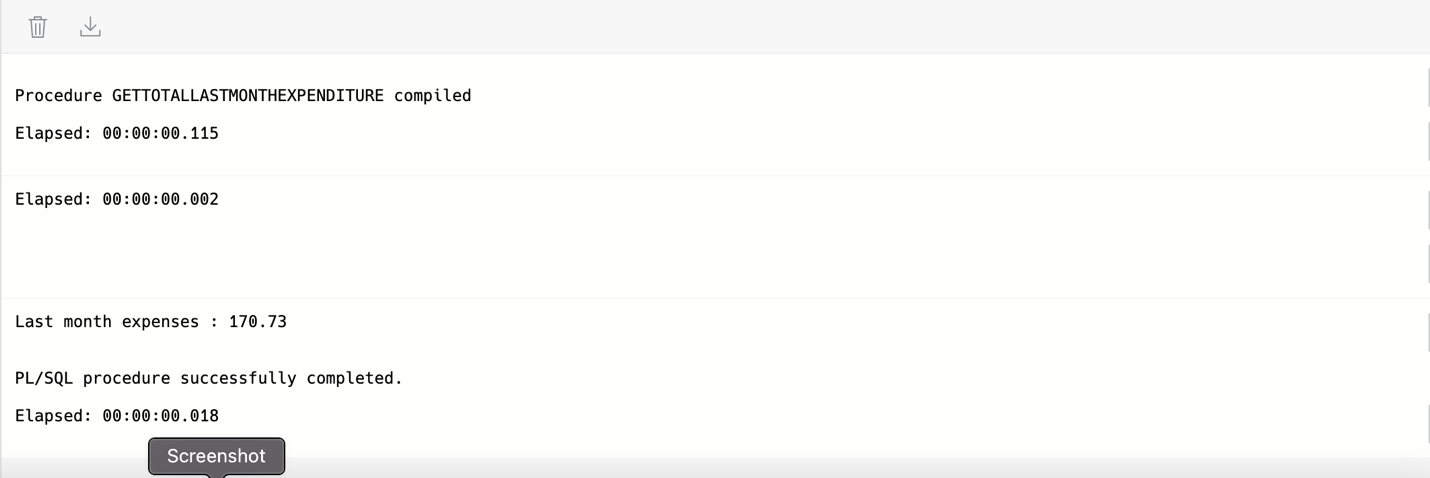
\includegraphics[scale=1]{figures/Picture22.png}
     \caption{Output for procedure-2}
     \label{fig:proc-2}
 \end{center}
\end{figure}

\end{enumerate}

\section{Triggers}
\begin{enumerate}
    \item A trigger to check if a discount coupon code entered by a customer is valid on before placing the order (Validate a coupon before placing an order). \\ \textbf{NOTE:} Here procedure-1 is used.
    \begin{lstlisting}
CREATE or REPLACE TRIGGER check_coupon_validity
BEFORE INSERT ON ORDERS
FOR EACH ROW
DECLARE
    thisvalidFrom Coupon.validFrom%TYPE;
    thisvalidThrough Coupon.validThrough%TYPE;
    thisvalidForXTimes Coupon.validForXTimes%TYPE;
    NUM_REDEMPTIONS Coupon.validForXTimes%TYPE;
BEGIN
SELECT c.validFrom, c.validThrough, c.validForXTimes 
INTO thisvalidFrom, thisvalidThrough, thisvalidForXTimes
FROM Coupon c
WHERE c.CouponCode = :NEW.CouponCode;
getNumRedemptions(:NEW.CouponCode, :NEW.PlacedBy, NUM_REDEMPTIONS);
IF (thisvalidFrom > SYSDATE) THEN
    Raise_Application_Error(-20000, 
    'Coupon code can be used on or after ' || thisvalidFrom);
ELSIF (thisvalidThrough < SYSDATE) THEN
    Raise_Application_Error(-20000, 'Coupon is expired');
ELSIF (NUM_REDEMPTIONS = thisvalidForXTimes) THEN
    Raise_Application_Error(-20000, 
    'Coupon code cannot be used. Maximum number of redemptions reached');
END IF;
END;
/
/* Following command is used for testing trigger-1*/
INSERT INTO orders
VALUES     (2011,
            sysdate,
            'Prepared',
            NULL,
            24.39,
            'vYh4x09z',
            4024007101499563,
            3,
            NULL,
            1,
            4001,
            3001,
            4,
            NULL,
            NULL,
            NULL,
            2,
            32391321226,
            NULL); 

    \end{lstlisting}
    \begin{figure}[H]
 \begin{center}
     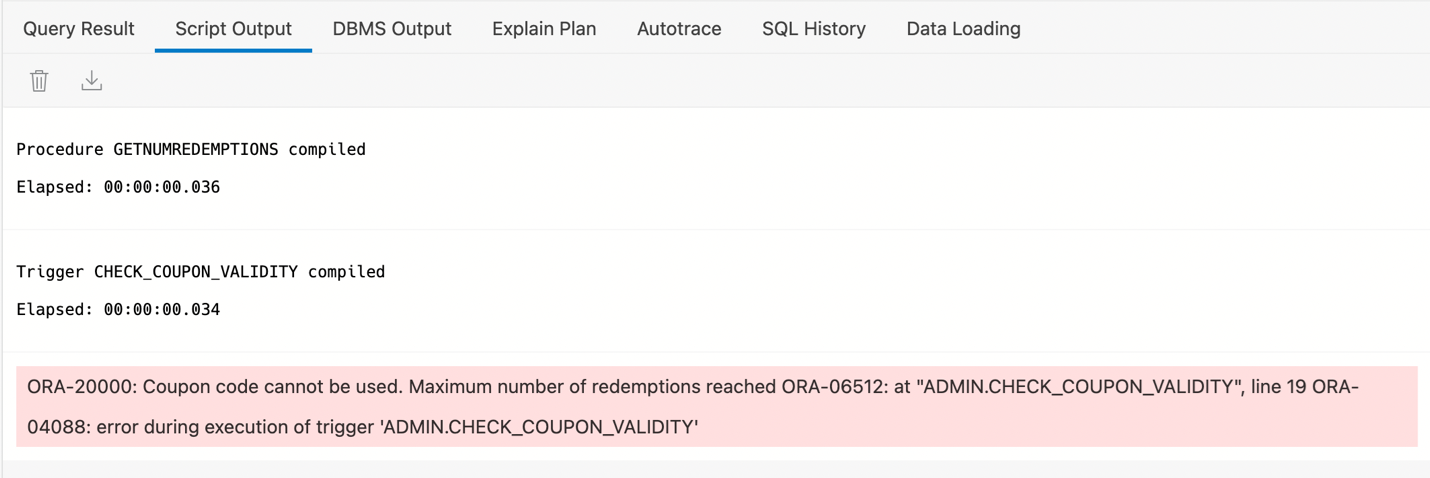
\includegraphics[scale=1]{figures/Picture21.png}
     \caption{Output of trigger-1 test}
     \label{fig:2b_graph_n}
 \end{center}
\end{figure}

\item Update the Pickup and Delivery time based on order status change i.e. A trigger to update the timings of a particular order id based on change in order status.
\begin{lstlisting}
CREATE OR REPLACE TRIGGER ORDER_UPDATE
BEFORE UPDATE OF Status on ORDERS
REFERENCING OLD AS old NEW AS new
FOR EACH ROW
BEGIN  
IF :old.Status = 'Prepared' AND :new.Status = 'Pickup' and UPDATING THEN
:new.PickUpTime := SYSDATE;
END IF;
IF :old.status = 'Pickup' AND :new.status = 'Delivered' and UPDATING THEN
:new.DeliveryTime := SYSDATE;
END IF;
END;
/

/* Following commands are used for testing trigger-2*/
-- Test-Command-1
UPDATE ORDERS SET status = 'Pickup' WHERE OrderID = 2001;
-- Test-Command-2
UPDATE ORDERS SET status = 'Delivered' WHERE OrderID = 2001;

\end{lstlisting}
\begin{figure}[H]
    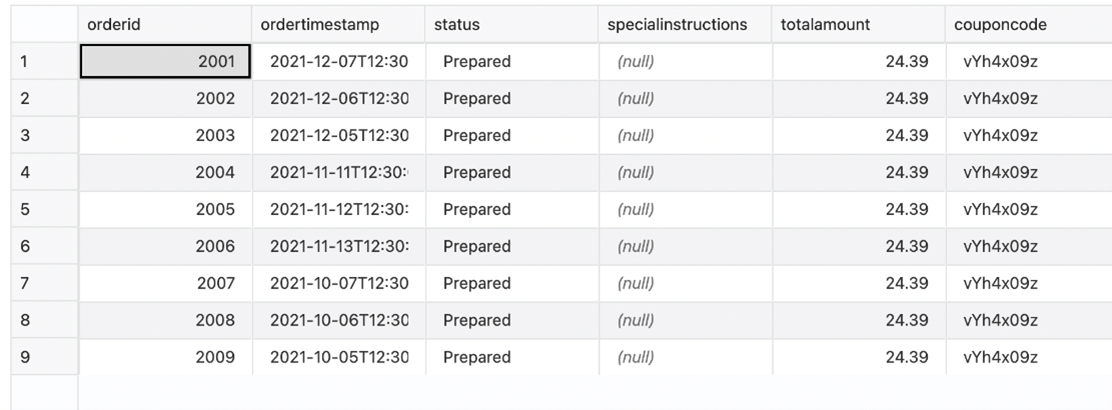
\includegraphics[width=\textwidth]{figures/Picture27.png}\hfill
    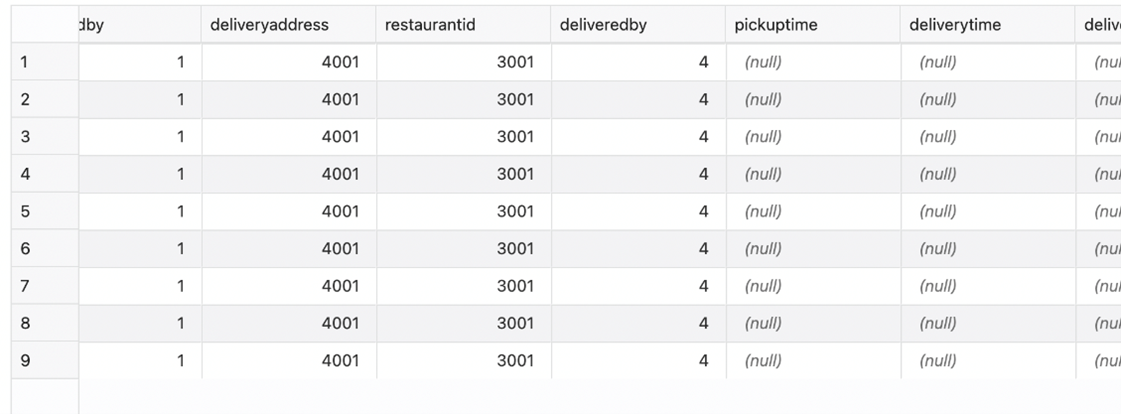
\includegraphics[width=\textwidth]{figures/Picture28.png}\hfill
    \\[\smallskipamount]
    \caption{Table state before running the trigger test commands-{1,2}.}\label{fig:trig21}
\end{figure}

\begin{figure}[H]
    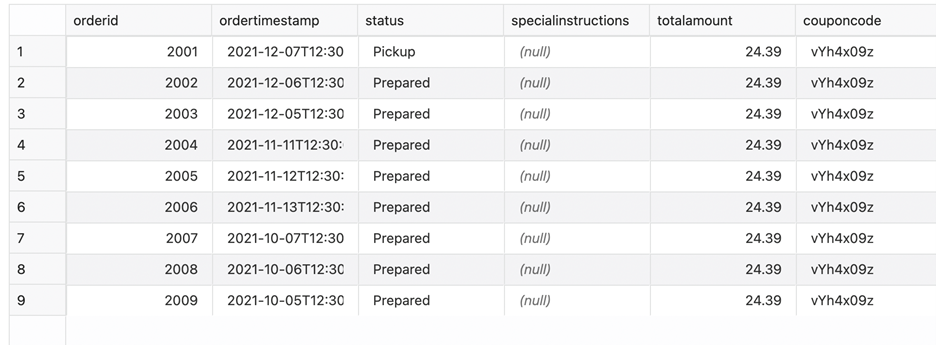
\includegraphics[width=\textwidth]{figures/Picture25.png}\hfill
    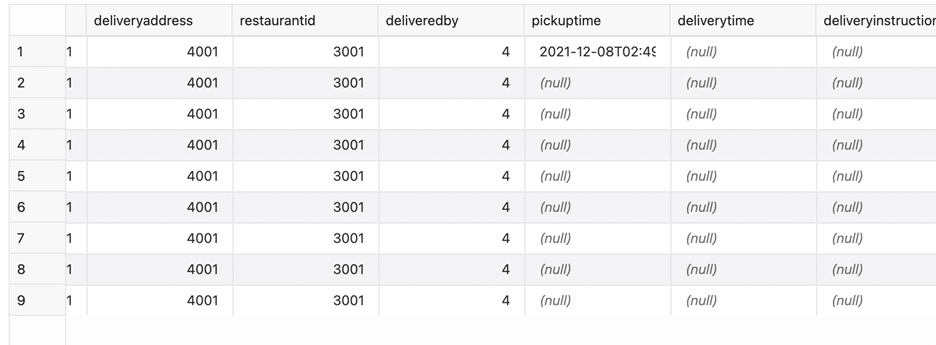
\includegraphics[width=\textwidth]{figures/Picture26.png}\hfill
    \\[\smallskipamount]
    \caption{Table state after running test-command-1.}\label{fig:trig22}
\end{figure}

\begin{figure}[H]
    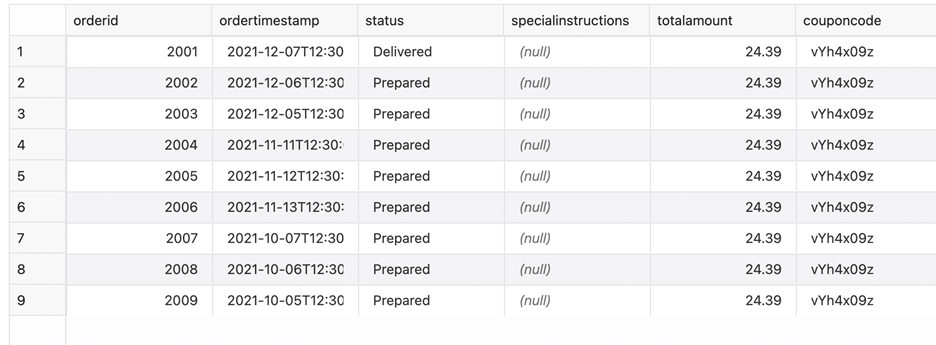
\includegraphics[width=\textwidth]{figures/Picture23.png}\hfill
    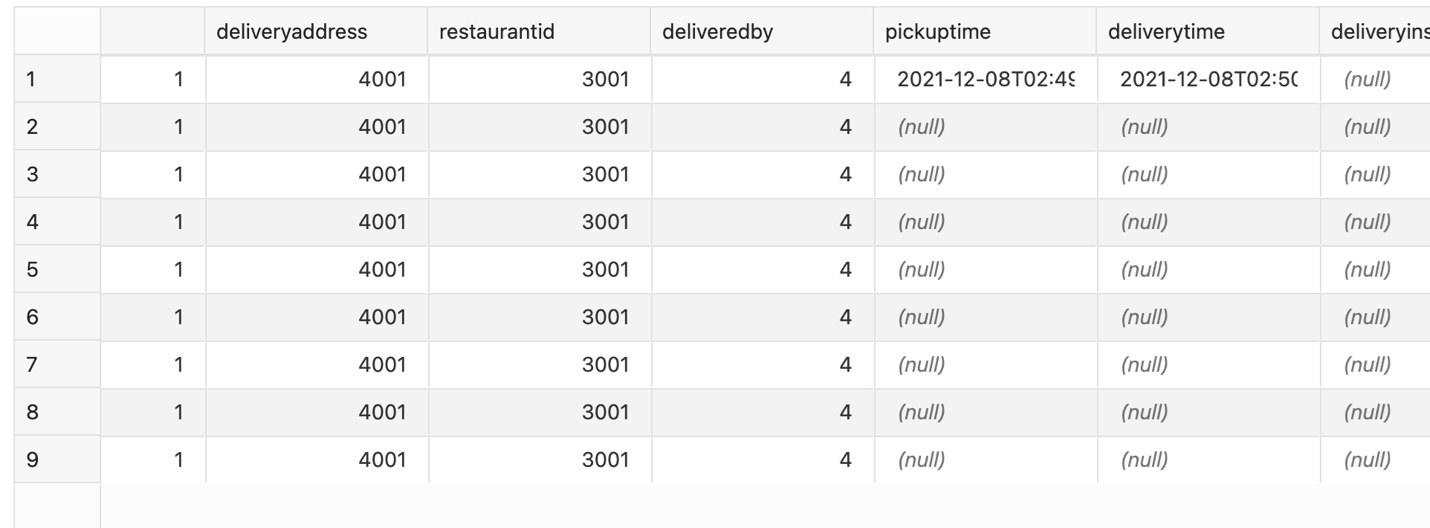
\includegraphics[width=\textwidth]{figures/Picture24.png}\hfill
    \\[\smallskipamount]
    \caption{Table state after running test-command-2.}\label{fig:trig22}
\end{figure}
\end{enumerate}

\end{document}


